\section{Experiments}
\label{sec:exp}

\subsection{Setup}
\label{sec:setup}
All models were trained and evaluated on one NVIDIA A100 (80\,GB) on Google Colab, with bf16 mixed precision. The supervised models (SID U-Net, Bridge U-Net and its ablations, DDBM-Feature) use AdamW with learning rate $2\times10^{-4}$, a 500-step warm-up, cosine decay to 2\%, batch 8, $512\times512$ packed crops and 40k iterations. MS-SSIM enters the loss after 20k iterations. Every 2k iterations we evaluate an EMA of the weights (decay 0.999) on 60 validation pairs (centre $512\times512$ packed crop), and we test the best validation checkpoint. The pixel-space DDBMs use learning rate $10^{-4}$ (1k-step warm-up, then constant), batch 16, $256\times256$ crops and are validated on 20 pairs with $N=10$ steps. Besides the fidelity metrics PSNR, SSIM and MS-SSIM we report LPIPS~\cite{zhang2018lpips} (AlexNet, lower is better) on the full-resolution images, a learned perceptual distance that, unlike PSNR, does not reward a blurry average. Unless stated otherwise, \textbf{test numbers are on all \SIDTESTPAIRS{} SID test pairs at full resolution} ($4256\times2848$), not on crops. Each configuration was trained once (one seed). To estimate run-to-run variation we retrained the SID U-Net with a second seed (Section~\ref{sec:sidres}).

One practical note: the first Bridge U-Net run diverged after 2.5k iterations (the loss jumped from 0.05 to 0.4 and never recovered). We restarted it and, for all runs, skip a batch whose loss exceeds five times the running average after the first 1k iterations (at most 10 in a row), which happened only a handful of times.

\subsection{SID: baseline, Bridge U-Net and ablations}
\label{sec:sidres}

\begin{table}[t]
\centering
\caption{SID Sony test set (\SIDTESTPAIRS{} full-resolution pairs). NFE: network evaluations per image; time: seconds per full-resolution image on an A100 (network only). LPIPS was added after the first set of checkpoints was lost, so it is measured on retrained copies ($^\dagger$: same configuration and seed; the copies score 28.61, 27.97 and 27.88\,dB PSNR, within 0.06\,dB of the original runs). The best value per column is in bold.}
\label{tab:sid}
\small
\resizebox{\linewidth}{!}{%
\begin{tabular}{@{}lrrccccr@{}}
\toprule
Model & Params & NFE & PSNR$\uparrow$ & SSIM$\uparrow$ & MS-SSIM$\uparrow$ & LPIPS$\downarrow$ & Time (s) \\
\midrule
SID U-Net, reported in~\cite{chen2018sid} & 7.8M & 1 & 28.88 & 0.787 & -- & -- & -- \\
SID U-Net (ours) & \PSID & 1 & 28.62 & 0.796 & \textbf{0.876} & \SIDRELPIPS$^\dagger$ & \TSID \\
SID U-Net (ours, second seed) & \PSID & 1 & \SIDRERUNPSNR & \SIDRERUNSSIM & \SIDRERUNMS & -- & \\
\midrule
Bridge U-Net (FiLM + distillation) & \PBRIDGE & 1 & 28.36 & 0.789 & 0.868 & -- & \TBRIDGE \\
\quad w/o distillation & \PBRIDGE & 1 & \textbf{28.94} & \textbf{0.798} & \textbf{0.876} & -- & \TBRIDGE \\
\quad w/o FiLM & \PNOFILM & 1 & 28.11 & 0.787 & 0.868 & -- & \TNOFILM \\
\midrule
DDBM-Feature, iterative ($N=3$) & \PFEAT & 4 & 18.02 & 0.449 & 0.742 & -- & \TFEATTHREE \\
DDBM-Feature, single pass & \PFEAT & 1 & 25.51 & 0.733 & 0.841 & -- & \TFEATZERO \\
DDBM, simplified, $N=5$ & \PDDBM & 5 & 28.03 & 0.782 & 0.862 & \textbf{\DDBMREFIVELPIPS}$^\dagger$ & \TDDBMFIVE \\
DDBM, simplified, $N=10$ & \PDDBM & 10 & 27.90 & 0.779 & 0.856 & \textbf{\DDBMRETENLPIPS}$^\dagger$ & \TDDBMTEN \\
DDBM, simplified, $N=10$, $\eta=0$ & \PDDBM & 10 & 27.88 & 0.776 & 0.854 & -- & \TDDBMTEN \\
DDBM, simplified, $N=20$ & \PDDBM & 20 & 27.77 & 0.776 & 0.851 & -- & \\
DDBM, released recipe, $\sigma_{\max}=1$, $N=5$ & \PDDBM & 14 & \SONEFIVEPSNR & \SONEFIVESSIM & \SONEFIVEMS & \SONEFIVELPIPS & \TOFFFIVE \\
DDBM, released recipe, $\sigma_{\max}=1$, $N=10$ & \PDDBM & 29 & \SONETENPSNR & \SONETENSSIM & \SONETENMS & \SONETENLPIPS & \TOFFTEN \\
DDBM, released recipe, $\sigma_{\max}=1$, $N=20$ & \PDDBM & 59 & \SONETWENTYPSNR & \SONETWENTYSSIM & \SONETWENTYMS & \SONETWENTYLPIPS & \\
\bottomrule
\end{tabular}}
\end{table}

Table~\ref{tab:sid} gives the main results. Our SID U-Net reaches 28.62\,dB, 0.26\,dB below the original paper~\cite{chen2018sid} and with a higher SSIM. The paper trains for 4000 epochs and we train for 40k iterations of batch 8, so the reproduction is faithful. A second training run with a different seed gives \SIDRERUNPSNR\,dB (SSIM \SIDRERUNSSIM), a difference of only \SIDSEEDGAP\,dB on the test set (33.07 vs.\ 32.89\,dB on validation). Two runs are a weak estimate of the variance, but they suggest that the test-set gaps of 0.25\,dB and more discussed below are not run-to-run noise.

\paragraph{The bridge module.} With both FiLM and distillation, the Bridge U-Net (28.36\,dB) is slightly \emph{worse} than the baseline. The ablations show why. Removing FiLM costs a further 0.25\,dB, so conditioning on exposure ratio and noise level helps. Removing distillation \emph{gains} 0.58\,dB, and the Bridge U-Net without distillation is the best model of this report: 28.94\,dB, +0.32\,dB over the baseline. The same order holds on the validation set (33.17 vs.\ 33.07\,dB for SID and 32.35\,dB with distillation). The distillation loss itself stays small, around $3\times10^{-4}$ in cosine distance: the encoder already maps the amplified short exposure and the long exposure to features of nearly the same direction. The loss therefore does little to clean the features. What it does do is pull the output of the bridge blocks back towards the plain encoder features, which removes most of the freedom the bridge was added for. In our setting, teacher-latent distillation is a regulariser that hurts.

\subsection{Diffusion bridges}
\label{sec:ddbmres}

\begin{figure}[t]
\centering
\begin{tikzpicture}
\begin{axis}[width=0.95\linewidth, height=5.2cm, xlabel={training iteration}, ylabel={val PSNR (dB)},
  xmin=0, xmax=60000, ymin=10, ymax=34, grid=major, grid style={gray!25},
  legend pos=south east, legend style={font=\footnotesize}, scaled x ticks=false,
  xtick={0,10000,20000,30000,40000,50000,60000}, xticklabels={0,10k,20k,30k,40k,50k,60k}]
\addplot[black, thick, mark=none] table[x=step,y=psnr] {data/val_sid.dat};
\addplot[blue, thick, mark=none] table[x=step,y=psnr] {data/val_ddbm.dat};
\addplot[red, thick, mark=none] table[x=step,y=psnr] {data/val_ddbm_official.dat};
\addplot[orange, thick, mark=none] table[x=step,y=psnr] {data/val_ddbm_official_s1.dat};
\legend{SID U-Net, DDBM simplified, DDBM released $\sigma_{\max}=80$, DDBM released $\sigma_{\max}=1$}
\end{axis}
\end{tikzpicture}
\caption{Validation PSNR during training (20--60 SID validation pairs, centre crops, $N=10$ sampling steps for the DDBMs). With the released noise scale $\sigma_{\max}=80$ the DDBM learns very slowly. Matching the noise scale to the data ($\sigma_{\max}=1$) speeds up training a lot, but after 60k iterations the recipe still trails the simplified DDBM by about 4\,dB on validation (27.0 vs.\ 31.2--31.4\,dB).}
\label{fig:valcurves}
\end{figure}

\paragraph{DDBM-Feature does not work as a diffusion model.} The feature-space variant of the original project reaches 25.51\,dB when it is run as a single pass at $t=0$, i.e.\ as a time-conditioned U-Net. Its intended iterative inference, which re-encodes its own output as the ``long exposure'' feature, collapses to 18.02\,dB. During training the decoder always sees features of the \emph{true} long exposure, while at test time it sees features of its own previous estimate, so errors compound from step to step. The longer we train, the more the decoder relies on these features: the validation PSNR of the iterative sampler peaks at 19.7\,dB after 6k iterations and falls to 12.3\,dB at 40k. A bridge whose endpoint is unavailable at test time cannot be sampled this way. This is why we implemented the pixel-space model, whose endpoint $x_T$ comes from the input itself.

\paragraph{A real DDBM is competitive but does not beat regression on PSNR.} The simplified pixel-space DDBM reaches 28.03\,dB with $N=5$ steps, 0.6\,dB below the SID U-Net, with twice the parameters and five times the compute. More sampling steps make it \emph{worse}: 27.90\,dB at $N=10$ and 27.77\,dB at $N=20$. This is expected. PSNR and SSIM reward the posterior mean, which is exactly what an $L_1$/$L_2$ regression network estimates. A diffusion model is trained to draw \emph{samples} from the posterior, and for an exact sampler the expected squared error of a sample is twice that of the posterior mean. Fewer steps behave more like a single denoising step and stay closer to the mean, so they score higher. The deterministic DBIM sampler ($\eta=0$) gives the same PSNR as the ancestral one. The possible benefit of diffusion, sharper texture instead of a blurry average, is not what these metrics measure.

\paragraph{On a perceptual metric the DDBM is better.} LPIPS reverses the order. The simplified DDBM scores \DDBMREFIVELPIPS{} against \SIDRELPIPS{} for the SID U-Net, 14\% lower, while being 0.6\,dB worse in PSNR. This is the perception--distortion trade-off~\cite{blau2018perception}: no estimator can be best on both, and the regression network sits at the low-distortion end. Unlike PSNR, LPIPS does not get worse with more steps ($N=5$ and $N=10$ give the same value), so the extra steps move the output away from the mean without making it look less like the target. The released recipe shows the same effect more strongly. From $N=10$ to $N=20$ its LPIPS improves from \SONETENLPIPS{} to \SONETWENTYLPIPS{}, almost reaching the simplified model, although its PSNR (\SONETWENTYPSNR\,dB) stays 2.4\,dB lower. The gain is modest in the crops of Fig.~\ref{fig:crops}: the simplified DDBM looks much like the U-Net, slightly less smooth in flat regions, and in the $\times250$ scene its colours drift towards yellow. Because LPIPS was measured on retrained copies, this comparison rests on one run per model.

\paragraph{The released recipe: the noise scale explains the slow start, not the gap.} Trained with its default $\sigma_{\max}=80$ for 60k iterations, the released DDBM recipe reached only 24.09\,dB on validation (SSIM 0.405), against 31.43\,dB for the simplified DDBM with the same network (Fig.~\ref{fig:valcurves}). Its validation PSNR stayed at about 12\,dB for the first 20k iterations. We traced this to the noise scale. Our images lie in $[-1,1]$, while the bridge noise at $\sigma=\sigma_{\max}/\sqrt2$ has a standard deviation of about 40, so in the middle of the bridge $x_\sigma$ is almost pure noise. And because $\sigma\sim\mathcal U(\sigma_{\min},\sigma_{\max})$, 99\% of the training samples have $\sigma>0.8$, so the low-noise range that decides the final detail is rarely trained. These settings come from image-to-image translation, where the two endpoints differ a lot. With $\sigma_{\max}=1$ and everything else unchanged, training is much faster: 21.4\,dB after 4k iterations and 25.85\,dB after 30k, against 12.5 and 17.0\,dB for $\sigma_{\max}=80$ at the same points. We then retrained it for the full 60k iterations, where it reaches \SONEVAL\,dB on validation, about 3\,dB above $\sigma_{\max}=80$ at the same point. The test score is still far below the simplified DDBM: \SONEFIVEPSNR, \SONETENPSNR{} and \SONETWENTYPSNR\,dB with $N=5$, 10 and 20, with low SSIM (\SONEFIVESSIM--\SONETWENTYSSIM). Two observations point to the sampler rather than the network. First, more steps help here, the opposite of the simplified model, and the gain has not levelled off at $N=20$. Second, the outputs keep visible residual noise and invented texture, and they are darker with a colour shift (Fig.~\ref{fig:crops}). With the stochastic churn step and the Karras schedule, a handful of steps does not remove the injected noise, while the simplified model's bridge posterior lands exactly on $\hat x_0$ in its last step. For restoration, where $x_T$ is already close to $x_0$, a small-noise bridge with a sampler that ends on the denoised estimate (I$^2$SB~\cite{liu2023i2sb}, our simplified model) is the better fit. The test evaluation of the $\sigma_{\max}=80$ model was lost when the cloud machine was reclaimed, so we report its validation score only.

\begin{figure*}[t]
\centering
\setlength{\tabcolsep}{1pt}
\begin{tabular}{ccccc}
\footnotesize Input (amplified) & \footnotesize SID U-Net & \footnotesize DDBM, simplified & \footnotesize DDBM, released, $\sigma_{\max}=1$ & \footnotesize Ground truth \\

\includegraphics[width=0.186\linewidth]{fig/0_input_amp.jpg} &
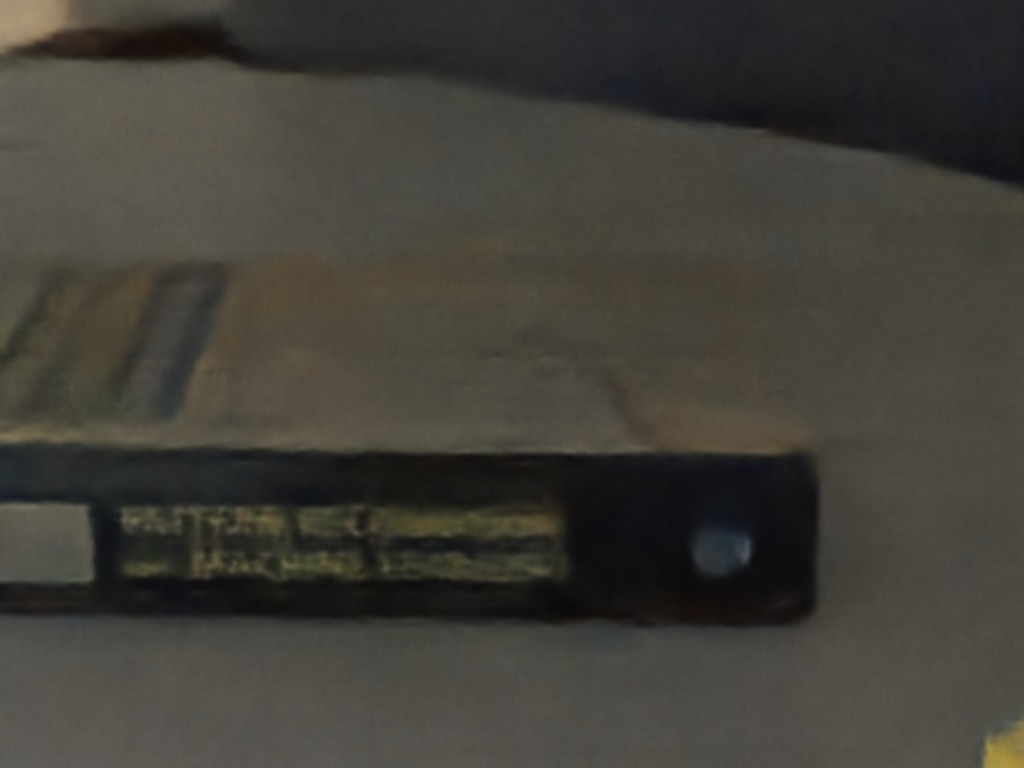
\includegraphics[width=0.186\linewidth]{fig/0_sid.jpg} &
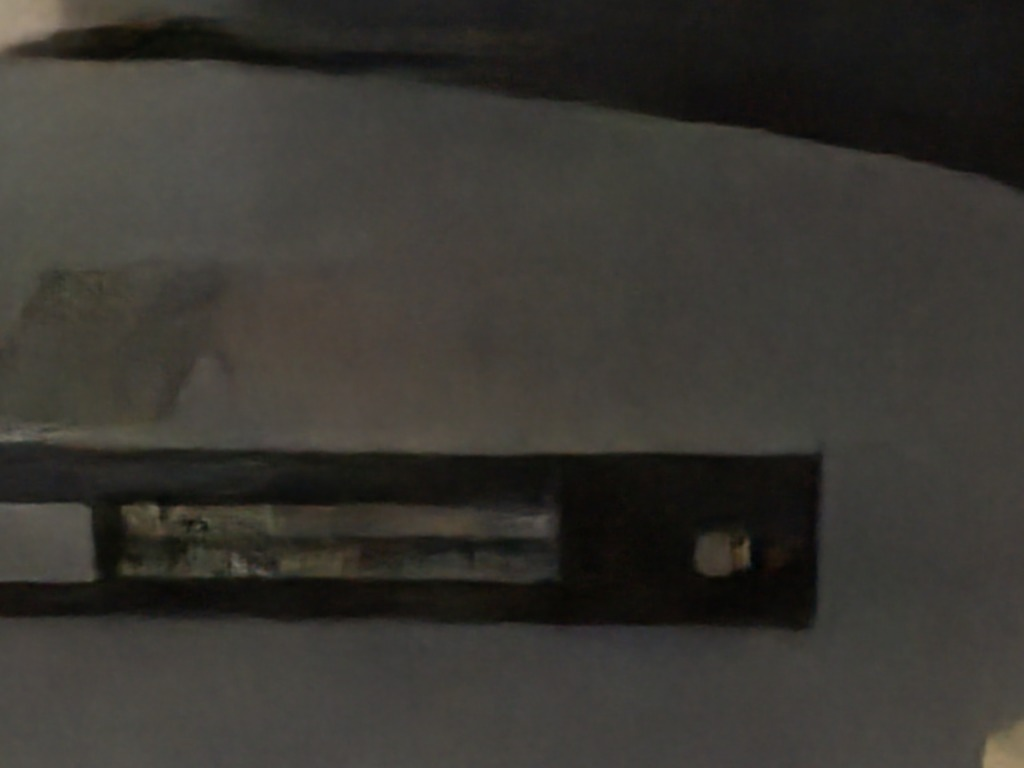
\includegraphics[width=0.186\linewidth]{fig/0_ddbm.jpg} &
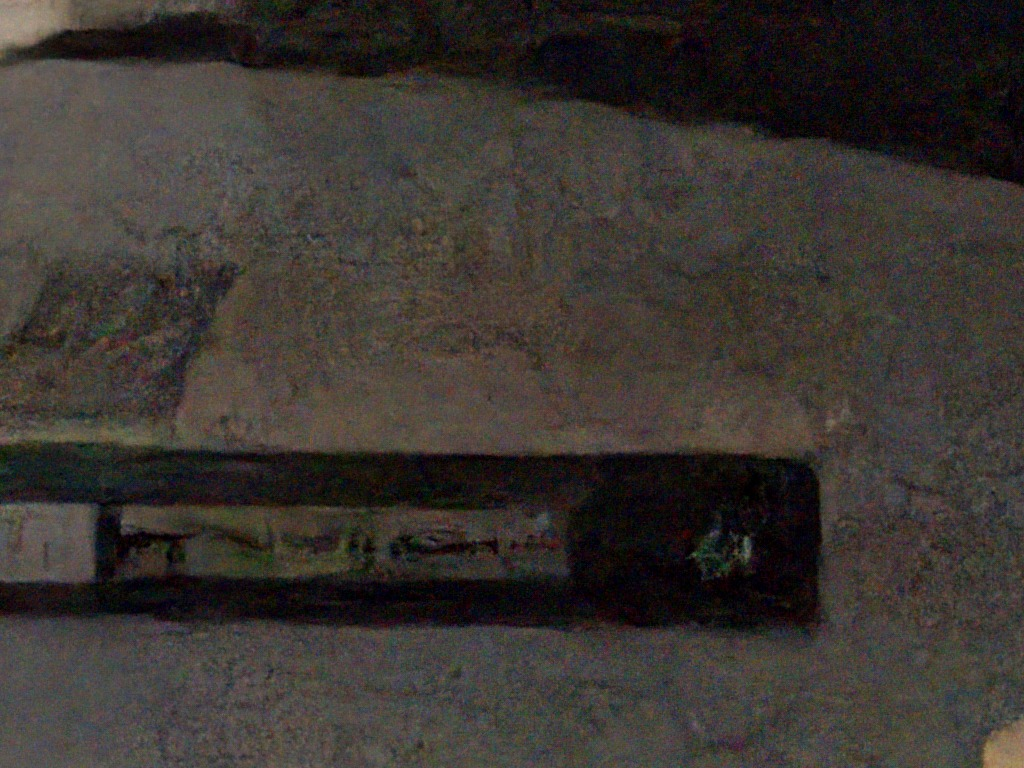
\includegraphics[width=0.186\linewidth]{fig/0_ddbm_official_s1.jpg} &
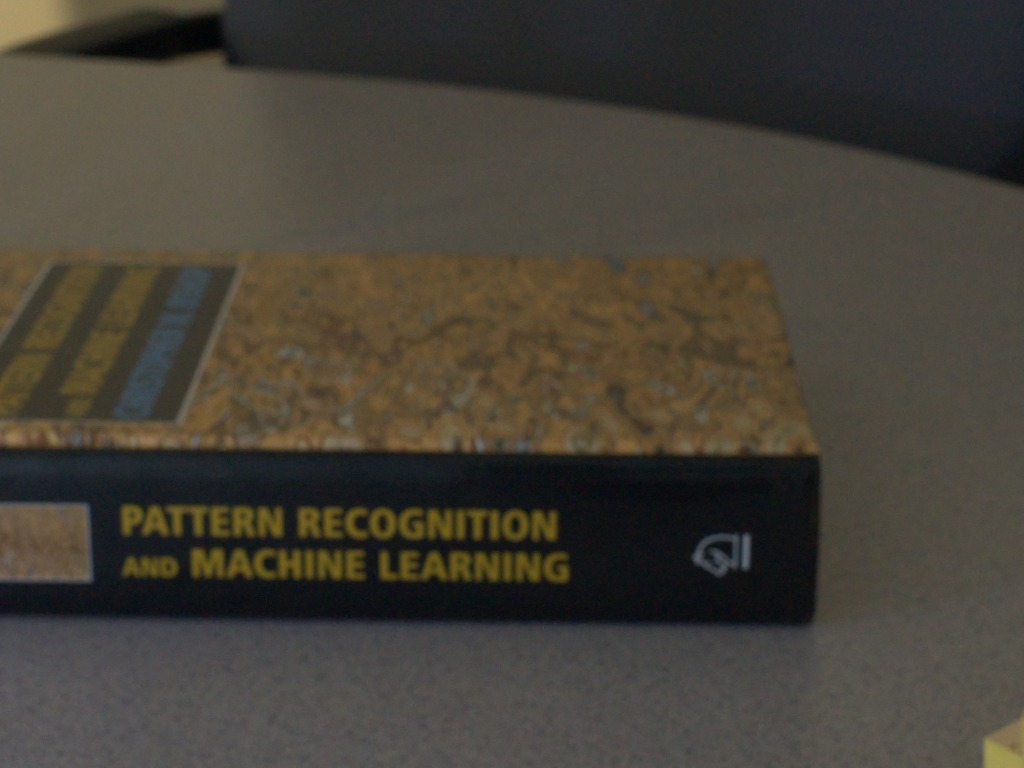
\includegraphics[width=0.186\linewidth]{fig/0_gt.jpg} \\
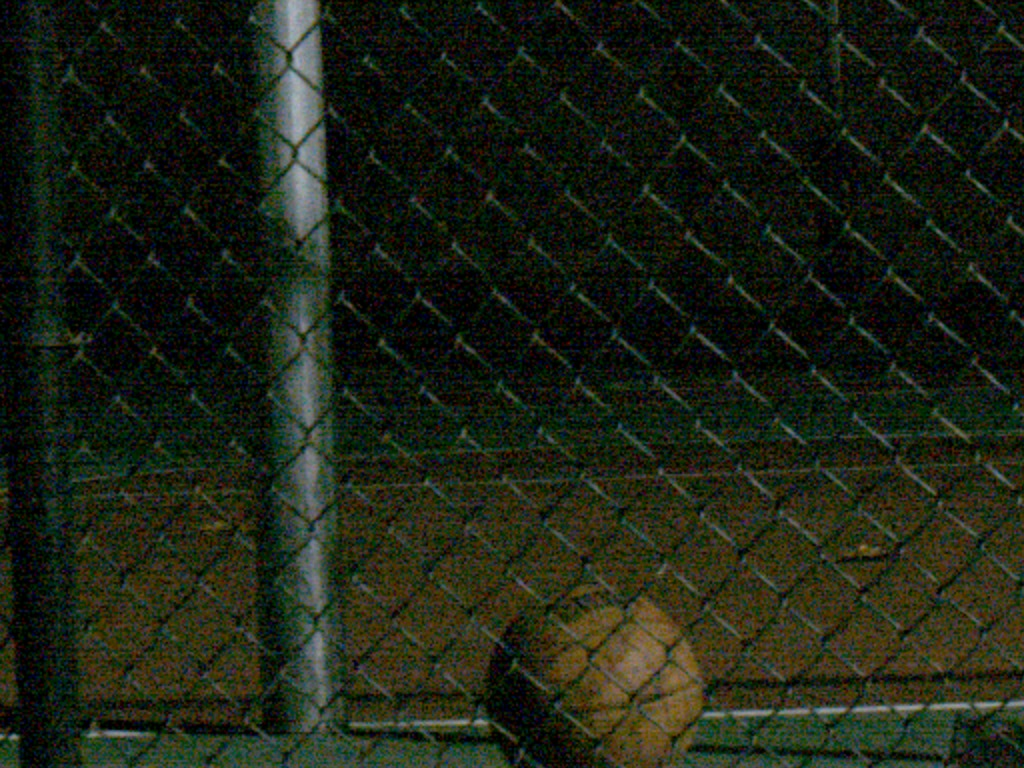
\includegraphics[width=0.186\linewidth]{fig/2_input_amp.jpg} &
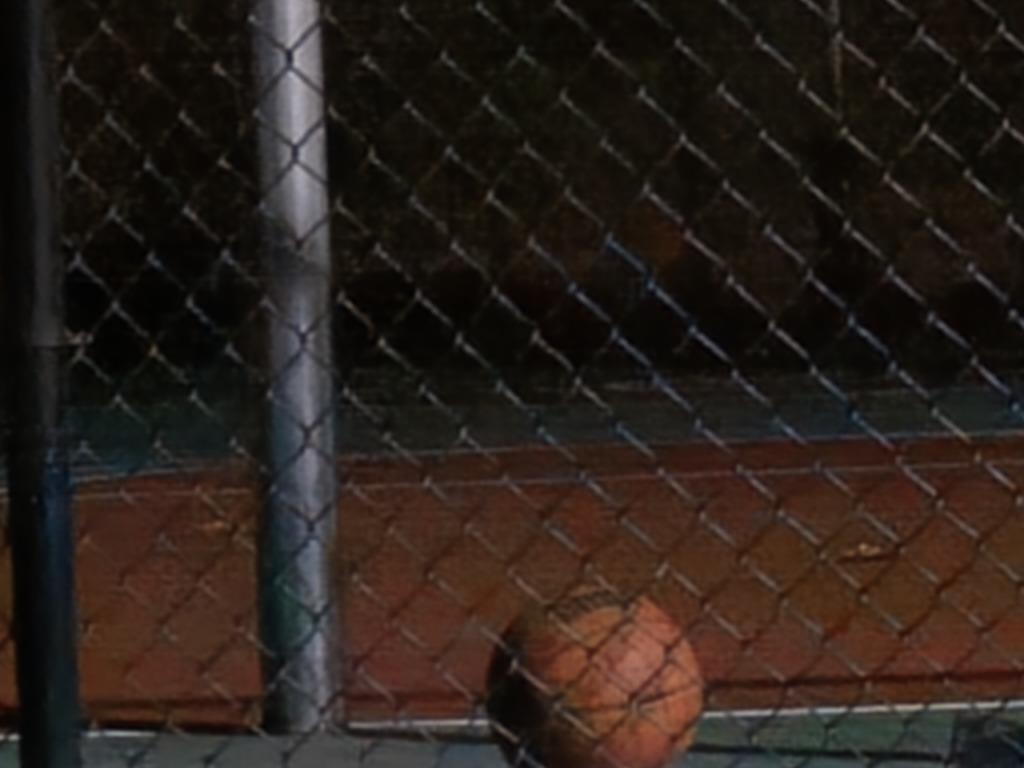
\includegraphics[width=0.186\linewidth]{fig/2_sid.jpg} &
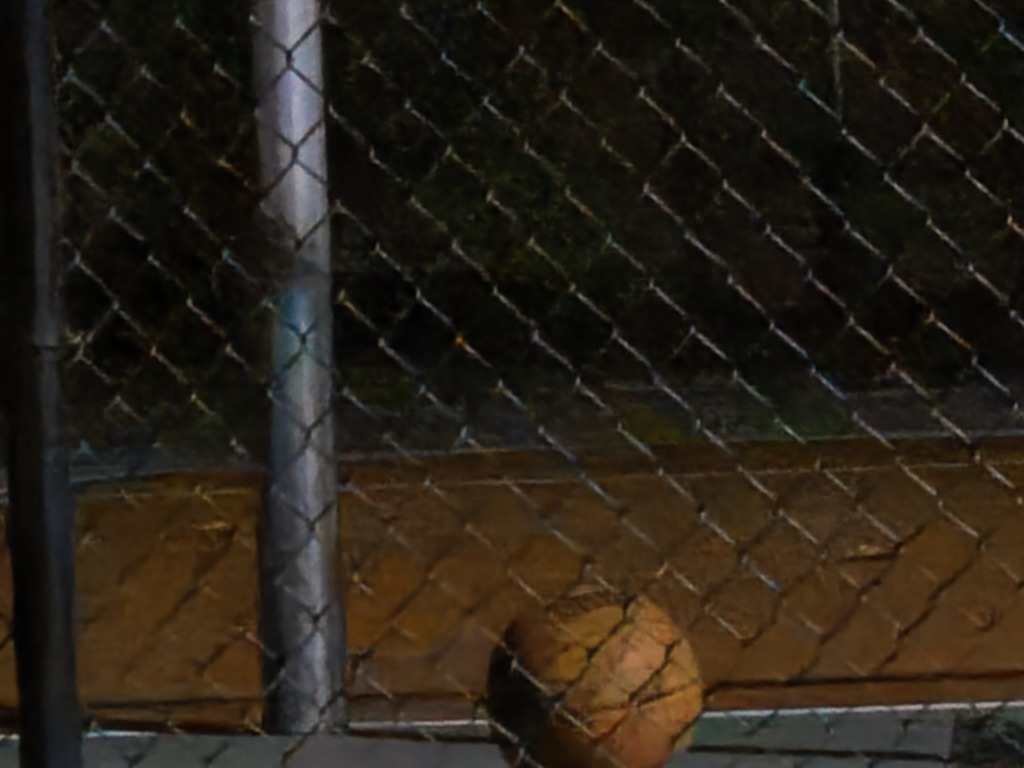
\includegraphics[width=0.186\linewidth]{fig/2_ddbm.jpg} &
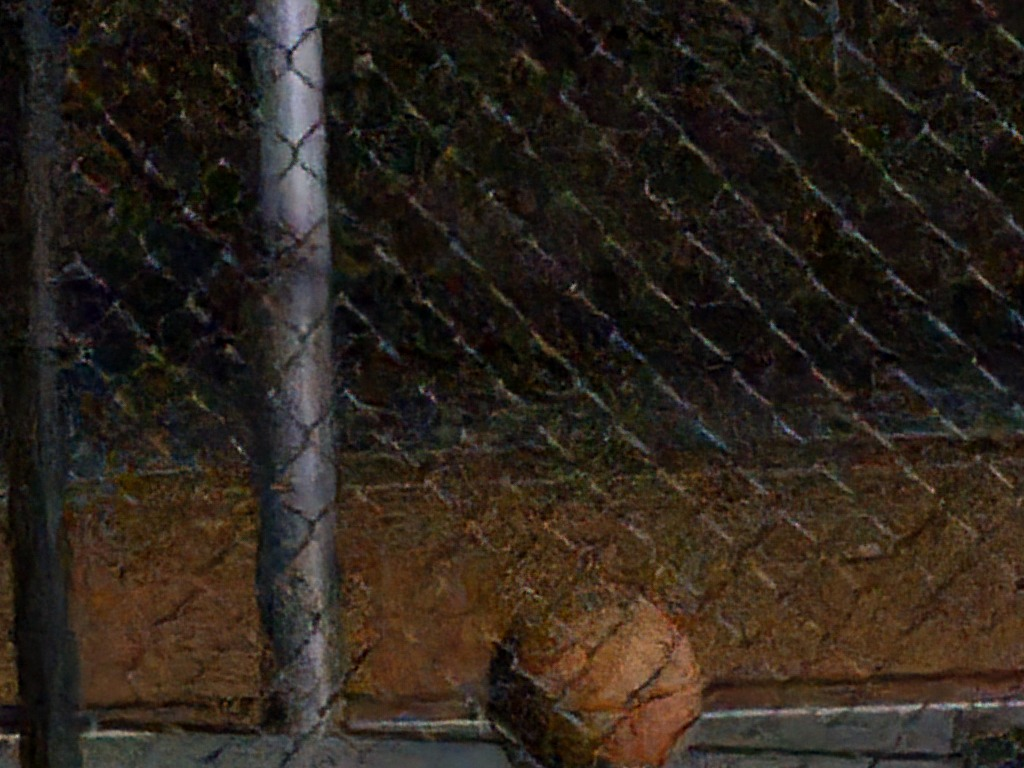
\includegraphics[width=0.186\linewidth]{fig/2_ddbm_official_s1.jpg} &
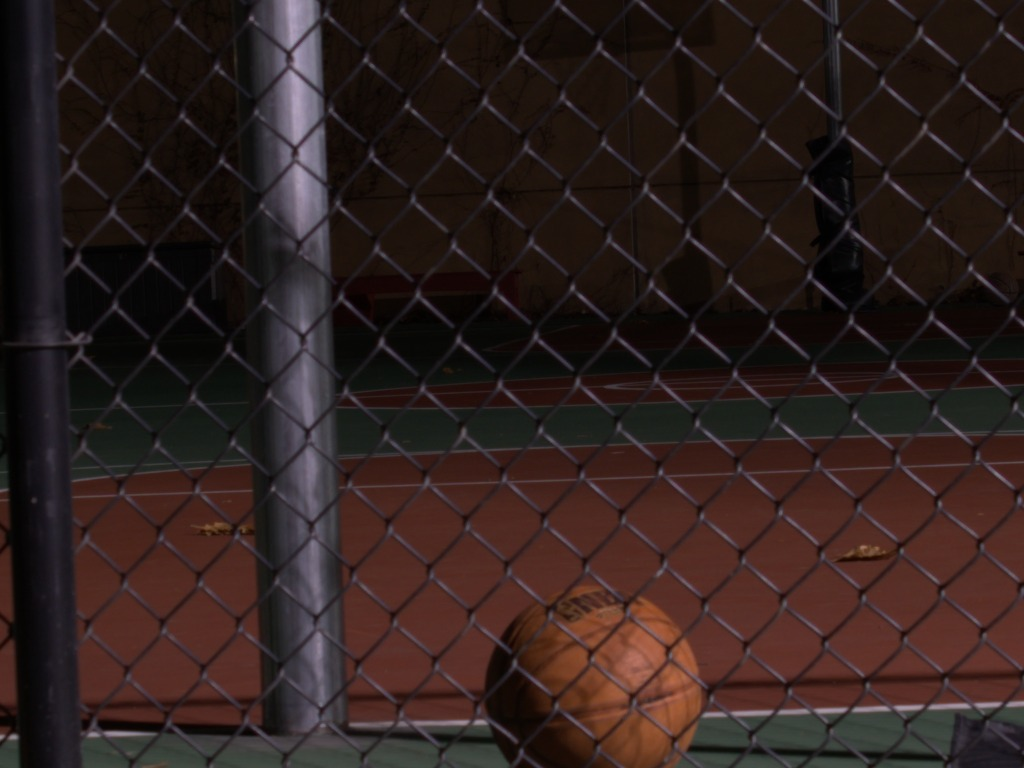
\includegraphics[width=0.186\linewidth]{fig/2_gt.jpg} \\
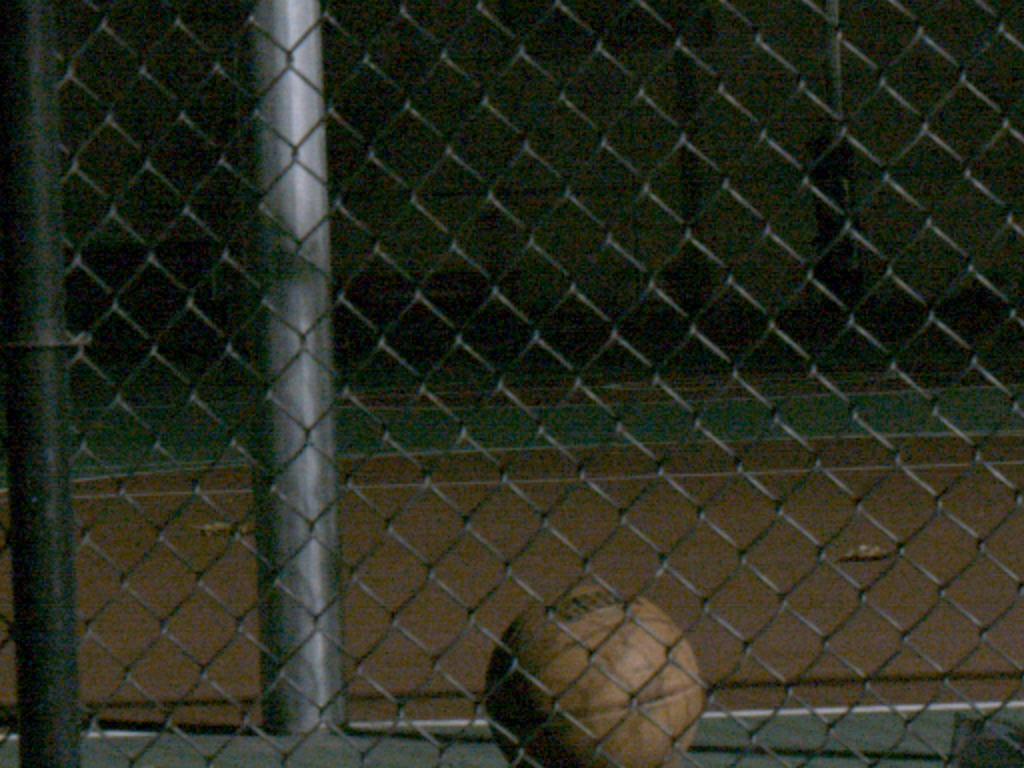
\includegraphics[width=0.186\linewidth]{fig/4_input_amp.jpg} &
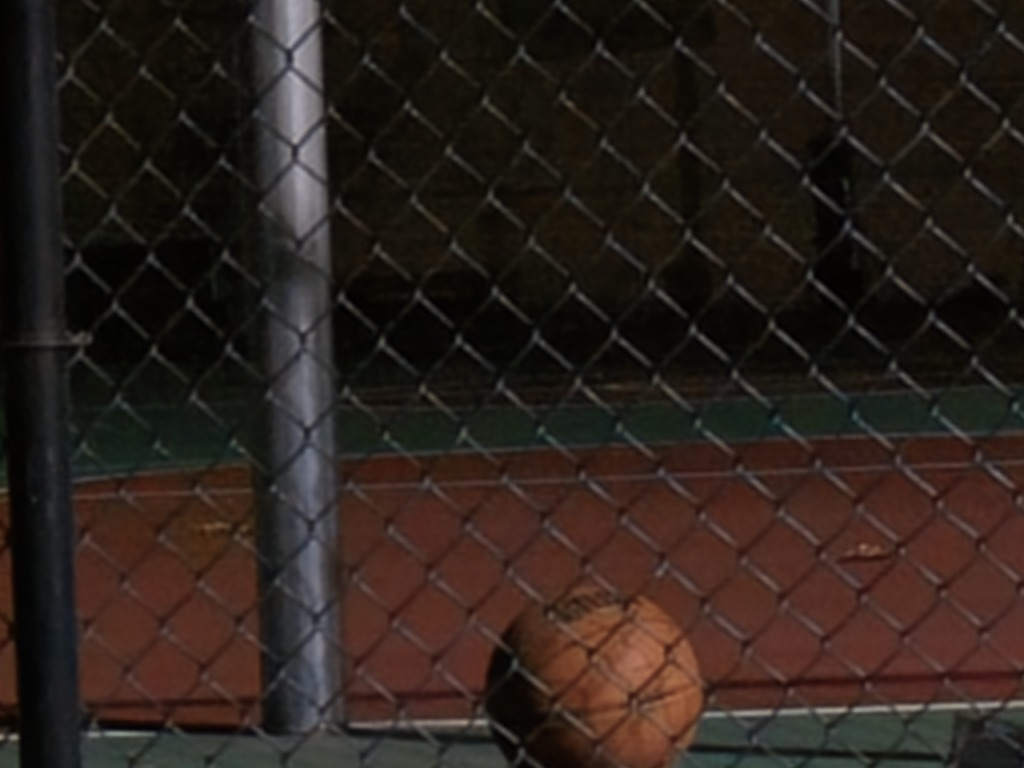
\includegraphics[width=0.186\linewidth]{fig/4_sid.jpg} &
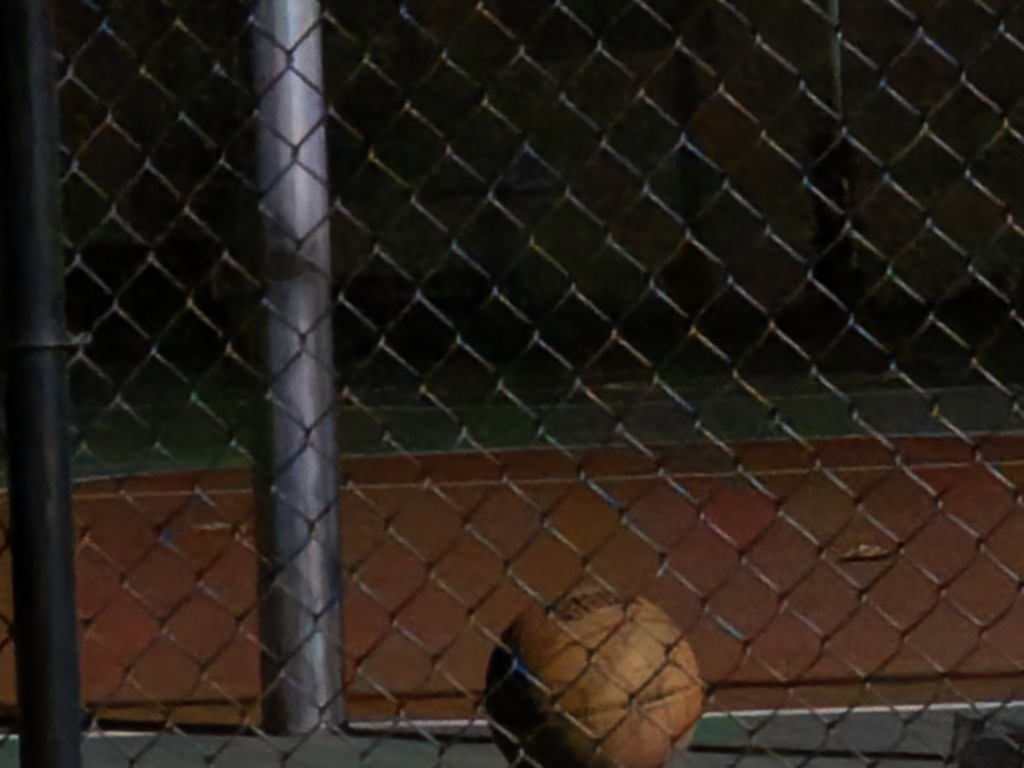
\includegraphics[width=0.186\linewidth]{fig/4_ddbm.jpg} &
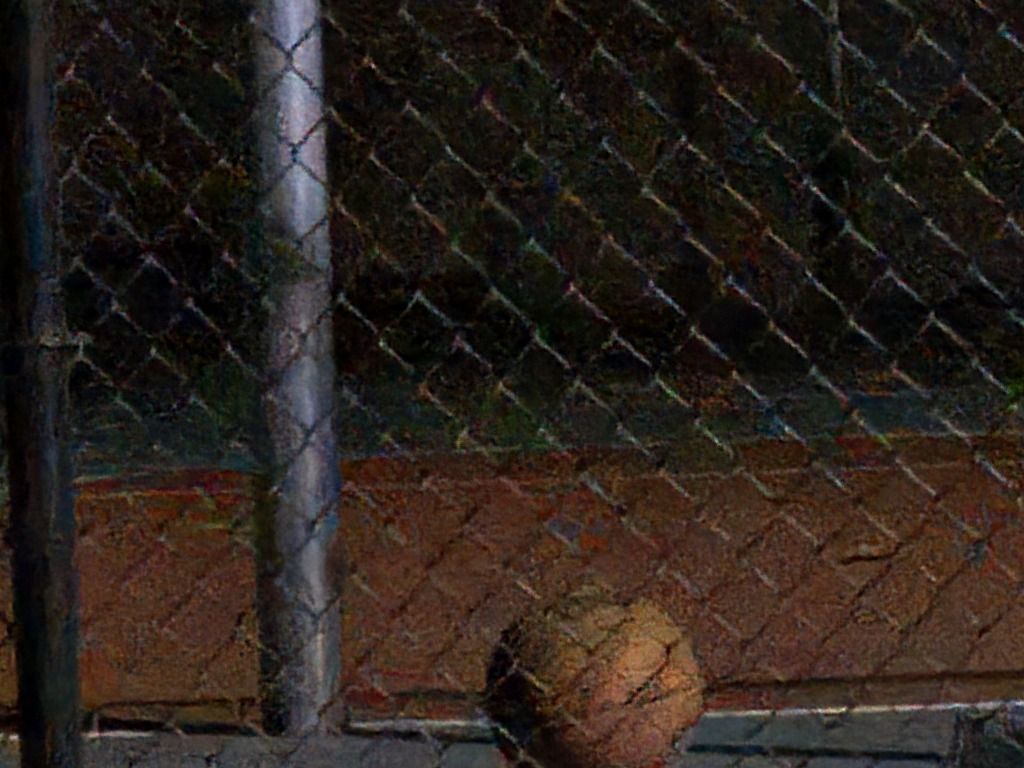
\includegraphics[width=0.186\linewidth]{fig/4_ddbm_official_s1.jpg} &
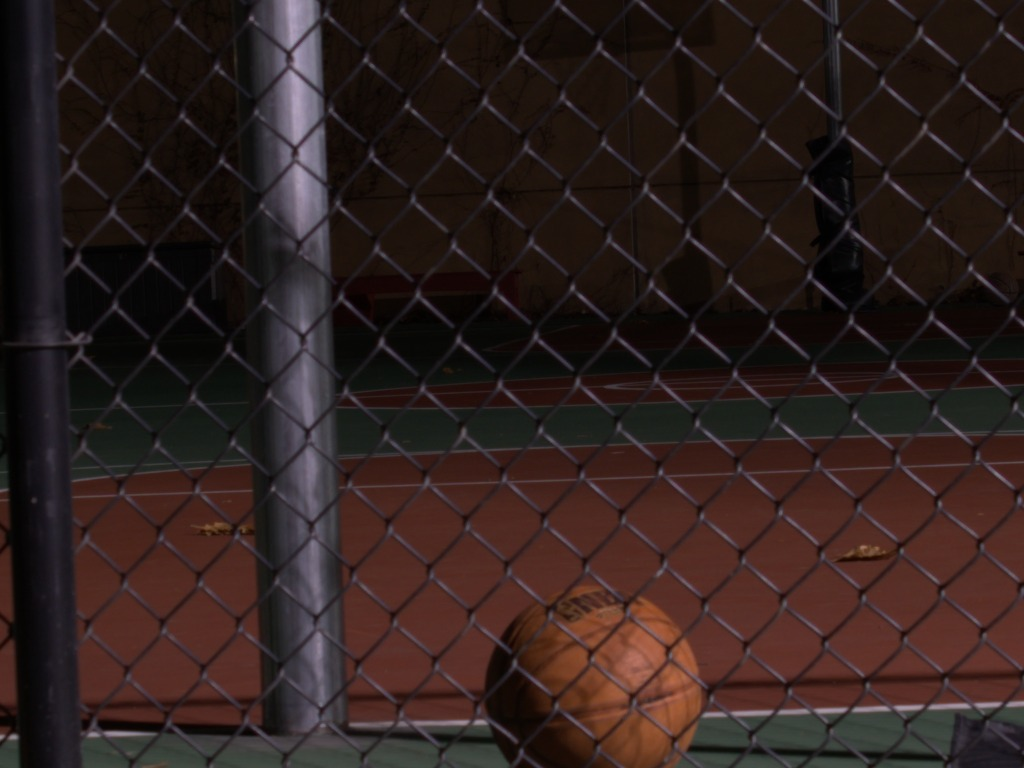
\includegraphics[width=0.186\linewidth]{fig/4_gt.jpg} \\
\end{tabular}
\caption{SID test crops ($1024\times768$ from the image centre) at exposure ratios $\times300$, $\times250$ and $\times100$ (top to bottom), from the models retrained after the first set of checkpoints was lost; both DDBMs use $N=10$ steps. The input is the amplified short exposure with a naive demosaic and white balance. The SID U-Net is smooth but faithful. The simplified DDBM is close to it, with a yellow colour drift in the middle row. The DDBM trained with the released recipe keeps residual noise, invents texture (the book cover) and is darker than the target.}
\label{fig:crops}
\end{figure*}

\subsection{Adapting to new cameras}
\label{sec:eldres}

\begin{table}[t]
\centering
\caption{ELD test scenes 7--10 ($\times100$ and $\times200$, 24 pairs per camera, $1024\times1024$ packed crops). PSNR / SSIM, starting from the SID-trained Bridge U-Net, which scores 24.37\,dB on average without adaptation. Fine-tuning uses all pairs of scenes 1--6 of the three cameras.}
\label{tab:eld}
\small
\begin{tabular}{@{}lcccc@{}}
\toprule
 & Canon 70D & Canon 700D & Nikon D850 & Mean \\
\midrule
Decoder + bridge & \textbf{26.16} / 0.740 & 25.99 / 0.709 & 29.35 / 0.811 & 27.17 / 0.753 \\
All layers & 26.14 / \textbf{0.745} & \textbf{26.01} / \textbf{0.713} & \textbf{29.81} / \textbf{0.827} & \textbf{27.32} / \textbf{0.762} \\
\bottomrule
\end{tabular}
\end{table}

\paragraph{Fine-tuning.} Without adaptation, the SID-trained model loses more than 4\,dB on the ELD cameras (24.37\,dB on average, against 28.4\,dB on SID). The other sensors have different colour responses and noise, and their frames span ratios down to $\times1$. Fine-tuning on the \ELDFTPAIRS{} pairs of scenes 1--6 recovers about 3\,dB (Table~\ref{tab:eld}): 27.32\,dB on average for all layers and 27.17\,dB with a frozen encoder. Freezing the encoder is almost as good on the two Canons and 0.46\,dB worse on the Nikon D850. Most of the camera-specific change can thus be absorbed by the decoder and the bridge, but low-level features still matter for a sensor that differs more from the Sony.

\begin{table}[t]
\centering
\caption{Few-shot adaptation on ELD: PSNR on scenes 7--10, averaged over the three cameras. $K$ adaptation scenes per camera, 12 pairs per scene. \emph{Adam}: 200 Adam steps (lr $2\times10^{-5}$); \emph{inner}: 30 SGD steps with the meta-training inner learning rate $10^{-3}$.}
\label{tab:fewshot}
\small
\begin{tabular}{@{}llcccc@{}}
\toprule
Initialisation & Adaptation & $K=0$ & $K=1$ & $K=3$ & $K=5$ \\
\midrule
SID U-Net & Adam & 24.17 & \textbf{26.74} & \textbf{27.36} & \textbf{27.54} \\
Bridge U-Net & Adam & 24.37 & 26.31 & 26.66 & 27.05 \\
Meta-learned Bridge & Adam & \textbf{24.77} & 26.48 & 26.86 & 27.15 \\
\midrule
Bridge U-Net & inner & -- & 24.40 & 24.53 & 24.25 \\
Meta-learned Bridge & inner & -- & \textbf{25.29} & \textbf{25.26} & \textbf{25.46} \\
\bottomrule
\end{tabular}
\end{table}

\paragraph{Few-shot adaptation and meta-learning.} Table~\ref{tab:fewshot} answers the second question. One scene of a new camera (12 pairs) already gives +1.7 to +2.6\,dB. Five scenes per camera (27.05--27.54\,dB) are as good as fine-tuning on six scenes of all three cameras (27.32\,dB). The meta-learned initialisation helps in two cases. It is the best model \emph{before} any adaptation ($K=0$: +0.40\,dB over the Bridge U-Net it started from and +0.60\,dB over SID), because meta-training on random sensor gains makes it robust to colour shifts. It is also clearly better when adaptation is as short as in meta-training (\emph{inner}: +0.9 to +1.2\,dB at every $K$). During meta-training the query loss after adaptation (L1 0.0459) was below the support loss before adaptation (0.0510), so the inner loop learned to adapt. With a long adaptation of 200 Adam steps, however, the advantage over the Bridge U-Net shrinks to 0.1--0.2\,dB, and the plain SID U-Net adapts best for every $K\ge1$. A good initialisation matters most when the adaptation budget is small. With more steps the initialisation matters less, and the smaller network (\PSID{} instead of \PBRIDGE{} parameters) adapts best from little data. The inner-loop adaptation does not improve with $K$, because 30 steps are too few to use more data.
